\section*{Exact Spectral Laws of Information}

For a centred Gaussian vector with covariance $\Sigma$, the differential entropy is $h=\tfrac12\log\det(2\pi e\Sigma)$. The mutual information between the blocks of a partition $x=(x_1,x_2)$ of dimensions $(p,r)$ is
\[
 I(\Sigma)=\frac12\log\frac{\det\Sigma_{11}\det\Sigma_{22}}{\det\Sigma}
 =-\frac12\sum_{k=1}^{p}\log(1-\rho_k^2),
\]
where $\rho_k$ are the population canonical correlations \citep{cover2006elements}. The Kullback--Leibler divergence between two centred Gaussians is $\KL(\N_A\|\N_B)=\tfrac12[\tr(B^{-1}A)-N-\log\det(B^{-1}A)]$. All three are smooth functions of the covariance matrix and are routinely estimated by substituting $S$ for $\Sigma$. I now derive the exact and asymptotic laws of these plug-in estimators. Proofs that are not given in the text are in Appendix~A.

\subsection*{Spurious mutual information}

Define the digamma partial sums $\Psi_n(k)=\sum_{i=1}^k\psi((n-i+1)/2)$ and the \emph{spurious information}
\begin{equation}
 B_n(p,r)=\tfrac12\bigl[\Psi_n(p)+\Psi_n(r)-\Psi_n(p+r)\bigr]
 =\tfrac12\sum_{i=1}^{r}\Bigl[\psi\Bigl(\frac{n-i+1}2\Bigr)-\psi\Bigl(\frac{n-p-i+1}2\Bigr)\Bigr].
 \label{eq:spurious}
\end{equation}
The second expression follows from the first by telescoping, and it is symmetric in $(p,r)$ although it does not look it.

\begin{proposition*}[Exact spurious information]
Let $n\geq p+r$ and let $\hat I=I(S)$ be the plug-in mutual information computed from $S=W/n$ with $W\sim\mathcal W_{p+r}(n,\Sigma)$. For every positive definite $\Sigma$,
\[
 \E\hat I=I(\Sigma)+B_n(p,r).
\]
The excess $B_n(p,r)$ is strictly positive whenever $p,r\geq1$, and it does not depend on $\Sigma$. The bias-corrected estimator $\tilde I=\hat I-B_n(p,r)$ is exactly unbiased for $I(\Sigma)$.
\end{proposition*}

The proof is two lines. The diagonal blocks satisfy $nS_{11}\sim\mathcal W_p(n,\Sigma_{11})$ and $nS_{22}\sim\mathcal W_r(n,\Sigma_{22})$ with the same number of degrees of freedom \citep[Ch.~3]{muirhead1982aspects}. Applying \eqref{eq:logdet} to each of the three determinants in $\hat I$ gives $\E\hat I-I=\tfrac12[\ell_n(p)+\ell_n(r)-\ell_n(p+r)]$, and the $\log(n/2)$ terms cancel because $p+r-(p+r)=0$. Positivity follows from the second form of \eqref{eq:spurious} and the strict monotonicity of $\psi$ on $(0,\infty)$. The Lean file proves the telescoping identity and the positivity for an arbitrary strictly antitone sequence. The analytic content is confined to \eqref{eq:logdet} and to the monotonicity of the digamma function. The independence of $B_n$ from $\Sigma$ is what makes the correction feasible. An analyst does not need to know the dependence in order to remove the bias that dimensionality adds to its estimate. Nothing in this argument requires $p$ and $r$ to be small. The same proposition holds after demeaning with $n-1$ in place of $n$, and after regressing both blocks on $k$ common regressors with $n-k$ in place of $n$. The second case is the version used for partial mutual information in the application.

When $\Sigma_{12}=0$ the full null law is available. In that case $\Lambda=\det S/(\det S_{11}\det S_{22})=\prod_k(1-\hat\rho_k^2)$ is Wilks' statistic, and $\hat I=-\tfrac12\log\Lambda$.

\begin{proposition*}[Null law]
If $\Sigma_{12}=0$ and $n\geq p+r$, then $\hat I\stackrel{d}{=}-\tfrac12\sum_{i=1}^p\log\beta_i$ with independent $\beta_i\sim\Beta\bigl(\tfrac{n-r-i+1}2,\tfrac r2\bigr)$. Consequently
\[
 \E_0\hat I=B_n(p,r),\qquad
 \Var_0\hat I=V_n(p,r)\equiv\frac14\sum_{i=1}^p\Bigl[\psi'\Bigl(\frac{n-r-i+1}2\Bigr)-\psi'\Bigl(\frac{n-i+1}2\Bigr)\Bigr].
\]
\end{proposition*}

The product representation of Wilks' $\Lambda$ is classical \citep[Ch.~8]{anderson2003introduction}, and the moments follow from $\E\log\beta=\psi(a)-\psi(a+b)$ and $\Var\log\beta=\psi'(a)-\psi'(a+b)$ for $\beta\sim\Beta(a,b)$. The two expressions for $\E_0\hat I$ agree by the telescoping in \eqref{eq:spurious}, which provides an internal consistency check. The null law gives an exact one-sided test of informational independence, rejecting when $(\hat I-B_n)/V_n^{1/2}$ exceeds a normal or exact quantile. It also provides an exact standard error for the corrected estimator under the null.

\subsection*{Proportional asymptotics and the Wachter law}

The finite-sample formulas have simple limits when both blocks grow with the sample. Let
\begin{align}
 \kappa(c_1,c_2)&=\tfrac12\bigl[(1-c_1-c_2)\log(1-c_1-c_2)-(1-c_1)\log(1-c_1)-(1-c_2)\log(1-c_2)\bigr],
 \label{eq:kappa}\\
 \nu(c_1,c_2)&=\tfrac12\log\frac{(1-c_1)(1-c_2)}{1-c_1-c_2}.
 \label{eq:nu}
\end{align}

\begin{proposition*}[Proportional limits]
Let $p/n\to c_1$ and $r/n\to c_2$ with $c_1,c_2>0$ and $c_1+c_2<1$. Then $B_n(p,r)/n\to\kappa(c_1,c_2)$ and $V_n(p,r)\to\nu(c_1,c_2)$. Under independence, $(\hat I-B_n(p,r))/V_n(p,r)^{1/2}$ converges in distribution to a standard normal. For every $\Sigma$, $\hat I/n-I(\Sigma)/n-\kappa(c_1,c_2)\to0$ in probability.
\end{proposition*}

The expansion $(1-c)\log(1-c)=-c+\sum_{k\ge2}c^k/[k(k-1)]$ gives the series
\begin{align*}
 \kappa(c_1,c_2)&=\frac12\sum_{k\geq2}\frac{(c_1+c_2)^k-c_1^k-c_2^k}{k(k-1)}
 =\frac{c_1c_2}2\Bigl(1+\frac{c_1+c_2}2+\cdots\Bigr),\\
 \nu(c_1,c_2)&=\frac12\sum_{k\ge2}\frac{(c_1+c_2)^k-c_1^k-c_2^k}{k}
 =\frac{c_1c_2}2\bigl(1+c_1+c_2+\cdots\bigr).
\end{align*}
All coefficients are positive, so $\kappa$ and $\nu$ are positive and increasing in each argument. The leading terms reproduce the classical fixed-dimension approximation $2n\hat I\approx\chi^2_{pr}$, with mean $pr/(2n)$ and variance $pr/(2n^2)$. The higher-order terms are the random matrix correction. They are not small. At $c_1=c_2=0.4$, the ratio $n\kappa/(pr/2n)$ equals $1.82$, so the classical formula misses almost half of the spurious information. Figure~\ref{fig:maps} maps $\kappa$ over the admissible region. The contours are hyperbola-like near the origin, where $\kappa\approx c_1c_2/2$, and steepen sharply as $c_1+c_2\to1$, where $(1-c_1-c_2)\log(1-c_1-c_2)$ has an infinite derivative.

\begin{figure}[htbp]
\centering
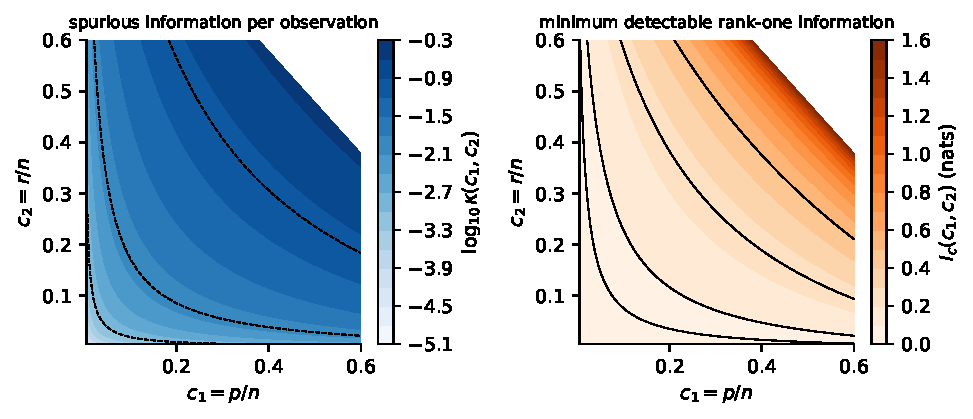
\includegraphics[width=\textwidth]{figures/theory_maps.pdf}
\caption{Left: spurious information per observation, $\kappa(c_1,c_2)$ from \eqref{eq:kappa}, on a logarithmic colour scale, with contours at $10^{-3}$, $10^{-2}$ and $10^{-1}$. Right: the minimum detectable rank-one information $I_c(c_1,c_2)$ from \eqref{eq:frontier}, with contours at $0.05$, $0.1$, $0.25$ and $0.5$ nats. Both are defined on $c_1+c_2<1$.}
\label{fig:maps}
\end{figure}

The plug-in information is also a linear spectral statistic of the canonical correlations, $\hat I=-\tfrac p2\int\log(1-x)\,\hat F_p(\dd x)$, with $\hat F_p$ the empirical distribution of $\hat\rho_1^2,\ldots,\hat\rho_p^2$. Under independence, $\hat F_p$ converges weakly to the Wachter law \eqref{eq:wachter}, whose support stays inside $[0,\omega_+]$ with $\omega_+<1$. Combining this with the previous proposition identifies a logarithmic moment of the Wachter law that does not appear to have been recorded before.

\begin{theorem*}[Logarithmic moment of the Wachter law]
For $0<c_1\leq c_2$ with $c_1+c_2<1$,
\begin{multline*}
 \int_{\omega_-}^{\omega_+}\log(1-x)\,w_{c_1,c_2}(x)\,\dd x=-\frac2{c_1}\,\kappa(c_1,c_2)\\
 =\frac1{c_1}\Bigl[(1-c_1)\log(1-c_1)+(1-c_2)\log(1-c_2)-(1-c_1-c_2)\log(1-c_1-c_2)\Bigr].
\end{multline*}
\end{theorem*}

The proof in Appendix~A computes the same almost sure limit of $\hat I/n$ in two ways, once through the Bartlett decomposition and once through the Wachter law. It needs only the convergence of the extreme canonical correlations to the edges of the support. Numerical quadrature confirms the identity to $10^{-13}$ over a grid of $(c_1,c_2)$, and the comparison in Figure~\ref{fig:wachter} shows how quickly the empirical spectrum settles on the Wachter law. The same reasoning, applied to the variance $V_n$, identifies $\nu(c_1,c_2)$ as the limiting variance of the linear statistic $\sum_k\log(1-\hat\rho_k^2)/2$, in line with the central limit theorems for Jacobi ensembles used by \citet{jiang2013central} and \citet{yang2015independence}.

\subsection*{Uninformative coordinates}

An important practical consequence is that spurious information can be manufactured. Suppose an analyst adds $m$ coordinates to the second block that are independent of everything else, so that the true mutual information is unchanged.

\begin{proposition*}[Monotonicity in uninformative coordinates]
For $m\geq1$, $n\ge p+r+m$ and every $\Sigma$,
\begin{multline*}
 \E\hat I_{p,r+m}-\E\hat I_{p,r}=B_n(p,r+m)-B_n(p,r)\\
 =\frac12\sum_{i=1}^{m}\Bigl[\psi\Bigl(\frac{n-r-i+1}2\Bigr)-\psi\Bigl(\frac{n-p-r-i+1}2\Bigr)\Bigr]>0.
\end{multline*}
In the proportional regime with $m/n\to c_3$, the increment per observation tends to $\kappa(c_1,c_2+c_3)-\kappa(c_1,c_2)$.
\end{proposition*}

The identity is again a telescoping sum, proved in the Lean file for an arbitrary sequence, together with strict positivity for a strictly antitone one. Its economic content is developed in the next section. The point to note here is that the digamma-corrected estimator is flat in $m$ by construction, whereas regularised plug-in estimators are not. Shrinking the covariance matrix towards a multiple of the identity, as \citet{ledoit2004well} do, or applying the rotationally invariant estimator \eqref{eq:rie}, removes spurious information. It also removes genuine information, and the numerical section shows that their estimates of $I$ collapse towards zero as $m$ grows. Covariance cleaning is optimised for quadratic losses on $\Sigma$, and information is not a quadratic functional.

\subsection*{The information cost of plug-in beliefs}

A Gaussian decision maker who adopts the plug-in law $\N(0,S)$ in place of $\N(0,\Sigma)$ incurs two natural information costs. The forward divergence $\KL(\N_\Sigma\|\N_S)$ is the expected excess log loss, or code length in nats, per future observation of using the estimated density for prediction. The reverse divergence $\KL(\N_S\|\N_\Sigma)$ is one half of Stein's loss of $S$ \citep{james1961estimation}. Write $\ell_n(N)$ for the exact log-determinant bias \eqref{eq:logdet}.

\begin{proposition*}[Exact information costs]
For $n\geq N+2$ and every $\Sigma$,
\begin{align*}
 \E\,\KL(\N_\Sigma\|\N_S)&=\frac12\Bigl[\frac{N(N+1)}{n-N-1}+\ell_n(N)\Bigr],&
 \E\,\KL(\N_S\|\N_\Sigma)&=-\frac12\ell_n(N).
\end{align*}
As $N/n\to q\in(0,1)$, the costs per dimension converge to $\tfrac12[q/(1-q)+\varphi(q)]$ and $-\tfrac12\varphi(q)$ respectively, with $\varphi$ from \eqref{eq:phi}.
\end{proposition*}

The forward formula uses $\E W^{-1}=\Sigma^{-1}/(n-N-1)$ \citep[Ch.~3]{muirhead1982aspects} and the algebraic identity $Nn/(n-N-1)-N=N(N+1)/(n-N-1)$, which is certified in Lean. Both costs expand as $q/4+O(q^2)$ per dimension, so that for small $q$ the total cost is close to the parameter count $N(N+1)/2$ divided by $2n$, the familiar Akaike penalty. For larger $q$ the forward cost explodes like $(1-q)^{-1}$, because the predictive density inherits the smallest sample eigenvalues and those approach zero at the left Marchenko--Pastur edge. The reverse cost stays bounded as $q\to1$, with limit $\tfrac12$ per dimension. For the empirical design used later, with $N=49$ industries and $n=249$ demeaned daily observations, the exact forward cost is \KLfwdN{} nats and the reverse cost \KLrevN{} nats. With a sixty-day window ($n=59$), they rise to \KLfwdSixty{} and \KLrevSixty{} nats. Expressed per future day, the forward costs are large compared with the daily information content of most signals that finance tries to measure. The forward cost is the information-theoretic counterpart of the out-of-sample penalty for minimum-variance portfolios. For $w=S^{-1}\one/\one^\top S^{-1}\one$ the exact ratios of in-sample and out-of-sample variance to the true minimum variance have expectations
\begin{equation}
 \E\frac{R_{\rm in}}{R}=\frac{n-N+1}n,\qquad
 \E\frac{R_{\rm out}}{R}=\frac{n-1}{n-N},
 \label{eq:gmv}
\end{equation}
whose product tends to $(1-q)^{-2}$ \citep{kan2007optimal,elkaroui2010high,bodnar2018estimation}. The first identity follows from $\one^\top\Sigma^{-1}\one/\one^\top W^{-1}\one\sim\chi^2_{n-N+1}$ \citep[Ch.~3]{muirhead1982aspects}, and both are confirmed numerically below.

\subsection*{A frontier for detectable information}

The proportional limits describe the bulk. The spiked theory \eqref{eq:cca-spike} describes what can be learned about a single dependence direction. Suppose the cross-block dependence has rank one, with canonical correlation $t$, so that $I(\Sigma)=-\tfrac12\log(1-t^2)$. The leading sample canonical correlation carries information about $t$ only if $t>t_c$. Define the \emph{information frontier}
\begin{equation}
 I_c(c_1,c_2)=-\frac12\log\bigl(1-t_c^2\bigr)=-\frac12\log\Bigl(1-\sqrt{\frac{c_1c_2}{(1-c_1)(1-c_2)}}\Bigr).
 \label{eq:frontier}
\end{equation}
Rank-one information below $I_c$ is real, in the sense that it changes the joint law and has positive economic value, but it is invisible to the spectrum. The leading canonical correlation converges to $\omega_+$ whatever the value of $t$. The aggregate statistic $\tilde I$ still responds, since its mean shifts by $I(\Sigma)$ while its null standard deviation is $\nu^{1/2}$, but it does not by itself locate the information. Locating it is the task of the leading canonical pair, which fails below the threshold. The right panel of Figure~\ref{fig:maps} shows that $I_c$ is negligible when both blocks are small relative to the sample, and becomes substantial when either block is large. For example, $I_c=0.091$ nats at $(c_1,c_2)=(0.1,0.2)$, and $I_c$ exceeds half a nat when $c_1+c_2$ approaches $0.8$ with balanced blocks. The frontier gives a precise meaning to the intuition that, in large cross-sections, some information is real but cannot be acted upon.
